\documentclass[
  utf8,%     More capable input encoding than latin-1.
  parskip,%  For vertical whitespace between paragraphs.  This comes down to more than just using parskip.sty, so it's better to use this class option.
  % S5MP % If you intend to really use margin paragraphs (not recommended!).
%  crop,%     Produce output with crop marks and paper size A4.  Liu-Tryck should like this.  Automatically adds information, including the physical page number, at the top of each page.
       %     Add option 'noInfo' to suppress the info at the top of each page when using option 'crop'.
  % Font options: 'kp' (default), 'times', 'lm'.  The KpFonts (loaded using 'kp'), is the most complete font among the provided options.  Among other, it supports slanted small caps.  See rtthesis.cls for more details regarding the font options.
  largesmallcaps,intlimits,widermath,% Good options to KpFonts.
  sharecounter,nobreak,definition=marks,%  See comments in the results chapter of this document for more information on these options!
  %numbers, % If you want to cite references by numbers, use this option.
  noparts% Use option 'noparts' if you do not make use of part divisions.
]{rtthesis}
\usepackage{xfrac}
\usepackage{breqn}
\usepackage{mythesis}
\usepackage{subfig}

\begin{document}
\selectlanguage{english}
\makeFrontPage
\frontmatter
\maketitle
%\makeLibraryPage{In this Bachelor’s thesis the following question is answered: Does the
inequality posed in the article Klyachko et al [2008] cover the real
part of the Bloch surface of a 3D quantum system when used as in Kochen
and Specker [1967]? The Klyachko inequality relies on using five
measurements to show contextuality of a subset of states on the real
part of the Bloch surface. These can now be used in several
configurations as present in the Kochen-Specker contextuality proof, by
simply rotating the measurements. We show here that these new
inequalities will have subsets of violation that eventually cover the
entire real part of the Bloch surface. This can be extended to show that
all states of a spin 1 system are non-contextual, so that we have
recovered a state-independent contextuality proof by using the Klyachko
inequality several times. In the final part, an interpretation of this is
given and also some recommendations for further research that should be
done in the field.}

%\begin{abstract}[swedish]
 % \input{svensk-sammanfattning}
%\end{abstract}
\begin{abstract}[english]
  In this Bachelor’s thesis the following question is answered: Does the
inequality posed in the article Klyachko et al [2008] cover the real
part of the Bloch surface of a 3D quantum system when used as in Kochen
and Specker [1967]? The Klyachko inequality relies on using five
measurements to show contextuality of a subset of states on the real
part of the Bloch surface. These can now be used in several
configurations as present in the Kochen-Specker contextuality proof, by
simply rotating the measurements. We show here that these new
inequalities will have subsets of violation that eventually cover the
entire real part of the Bloch surface. This can be extended to show that
all states of a spin 1 system are non-contextual, so that we have
recovered a state-independent contextuality proof by using the Klyachko
inequality several times. In the final part, an interpretation of this is
given and also some recommendations for further research that should be
done in the field.
\end{abstract}
%Blablabla said Nobody ~\cite{Nobody06} which.

\begin{acknowledgments}
A big thank you to my family and my fiancée whom have supported me throughout my education.
Another big thank you to my mentor Jan-Åke Larsson.

  \addvspace{1em}
  \begin{flushright}
    \textit{%
      Linköping, December 2013\\
      Patrik Hallsjö%
    }
  \end{flushright}
\end{acknowledgments}

\tableofcontents
%\begin{notation}% Passing the option "old" to the notation environment will redefine the notationtabular environment so that it produces an old style LaTeX tabular instead of a ctable.sty style tabular.
  \centering

  \begin{notationtabular}{Some mathematical notations}{Notation}{Meaning}
  
    $\identity_x$ & Identity matrix, with dimension x \\
    $\reals$ & Mängden av reella tal \\
    $\complexes$ & Mängden av komplexa tal \\
  \end{notationtabular}


\end{notation}
  

\mainmatter
\chapter{Introduction}\label{cha:intro}
What is given here is only meant to serve as a small introduction to some of the knowledge in physics which may be needed to understand this thesis.    
\newpage
\section{The main question in this thesis}
In this Bachelor's thesis the following question is of interest:\\
Does the inequality posed in the article \cite{PhysRevLett.101.020403} cover the real
part of the Bloch surface of a 3D quantum system when used as in~\cite{Kochen1968The}?\\
This will be done by evaluating the Klyachko inequality with the measurements produced by Kochen and Specker and then plotting this onto the Bloch sphere.
To understand the questions and how this will be done, some introduction is needed.\\
This topic was chosen in collaboration with my mentor for its interesting applications and also my interest in the field of contextuality. An interesting thing to note, in this field most discussion has been applied to spin 1/2 systems, and not any other system.
\section{Background of quantum mechanics}\label{sec:intro:Background of quantum mechanics}
Most of this section can be found in any university course in quantum mechanics. The material for this chapter has been based on the course given at Linköpings University with~\cite{Bransden:2000}
as the course literature. For more details consult the book. 
\subsection{The origin of quantum mechanics}
In the beginning of the 20th century, some physical phenomena could not be explained by classical physics, for example the ultra-violet disaster of any classical model of of black-body radiation, and the photoelectric effect. There were many other phenomena that were unexplainable, for more see for instance~\cite{Bransden:2000}.
It was these phenomena that led to the formulation of quantum mechanics, where energy transfer is quantized and particles can act as both waves and particles at the same time. Another big distinction between classical physics and quantum mechanics is that now it is more common to speak of statistical measurements, this is why quantum mechanics can be seen as an extension of statistical mechanics.
Statistical data such as the average value and the standard deviation is used to draw conclusions and compare several performed measurements on a system. A common operation in quantum mechanics is to take the statistical average known as the expectation value for a system.    

The most famous and by most considered the basic equation of quantum mechanics was discovered when E.\ Schrödinger was exploring the physics of small particles. A full derivation of this can be found in the original paper,~\cite{Schrodinger:1926}, or in a course of Analytical Mechanics. What he arrived at is known as the Schrödinger equation, with $\vec{x}$ as the position and t as the time, 
\begin{equation} \label{eq:Schrödinger}
i\hbar\frac{\partial}{\partial t}\psi (\vec{x}, t) = \hat{H}\psi (\vec{x}, t)
\end{equation}
which can be interpreted in the following way:
Since both i and $\hbar$ are constants, one can basically say that the time derivative of the wave-function is equal to the Hamiltonian of system acting on the wave-function. The Hamiltonian will not be discussed here, however it is a concept that is discussed a lot in the field of Analytical Mechanics.
It is the wave-function of a system that has the most interest in quantum mechanics. 
Not to forget, another important property of quantum mechanics is that nothing can be known about a system until it has been measured. It was this that was explained through the Schrödinger cat thought experiment. See more in the translation of the original paper ~\cite{Schrodinger:1980}.

Many new properties have been discovered through quantum mechanics, for instance that elementary particles and atoms have spin. Some more details can be found by studying classical angular momentum and how it continues in quantum mechanics. It is through this that the mathematics for spin is deduced. This will be discussed further in~\ref{sec:intro:Background of quantum mechanics:Finite dimentional quantum-states}
\subsection{Dirac bra-ket notation}\label{subsec:Dirac bra-ket notation}
By solving the Schrödinger equation, see equation (\ref{eq:Schrödinger}), a wave-function for a system can be found and utilized for calculations. From here on the wave-function will be denoted as a state: $|\psi\rangle$.
Here also the dependent variables are omitted for simplicity such that:
$$|\psi\rangle = \psi (\vec{x}, t)$$
This notation is known as the Dirac bra-ket notation, where the above is known as a ket-vector. Throughout this thesis the use of the word state and vector can be considered to be equal, since the state is represented as a vector in Hilbert space, see more in a course in functional analysis or~\cite{Kreyzig}. The bra-ket notation comes with certain notations, such as: $|\psi\rangle^\dagger = \langle\psi|$, the latter known as a bra-vector. Where $\dagger$ denotes the complex-conjugate. $\langle\psi|\psi\rangle =$ modulus of the vector $\psi$\\
Only a few details have been mentioned here. Using the bra-ket notation,~\ref{eq:Schrödinger} can be rewritten as: \begin{equation} \label{eq:Schrödinger2}
i\hbar\frac{\partial}{\partial t}|\psi\rangle = \hat{H}|\psi\rangle
\end{equation}
\subsection{Operator formalism}\label{sec:intro:Background of quantum mechanics:Operator formalism}
An observable corresponds to a value which can be measured, such as position, momentum, energy etc. Also, to be remembered from above, that in most cases, and in this thesis, conclusions can only be made from the expectation values of the observables. To note, there can be observables that can only be true or false. What is actually done is calculating the eigenvalues for the operators in Hilbert space. In the quantum mechanical framework, one utilizes so called operators to produce different observables. An example of this is the operator $\hat{x} = i\hbar\frac{\partial}{\partial p}$   
which when used or applied to a state will produce the position of the state.  So, mathematically to calculate the position would look something like this: $\langle\psi|\hat{x}|\psi\rangle$ 
\subsection{Commutating operators}
What does commutation mean?
Putting it simply, is is the ability to let two operators act after each other without the first one changing the result for the other. As an example: $\langle\psi|\hat{A}\hat{B}|\psi\rangle$ should produce the same value as $\langle\psi|\hat{B}\hat{A}|\psi\rangle$ if $\hat{A}$ and $\hat{B}$ commute. Subtracting these both should then equal zero. This is usually written as $[\hat{A},\hat{B}]$ where, to be evaluated should act on a state.
Some operators commute and some do not. A famous example of this is that the operator for momentum and position do not commute. So it is not possible to know the position and momentum of a state, for instance a particle, at the same time. It is from this one gets the Heisenberg uncertainty, see more details in~\cite{Bransden:2000}.

This is all a continuation of the fact that a measurement of a quantum-state will collapse the state, meaning that once a measurement has been done to the state, the simultaneous measurement of the second operator can not be accurately performed. Thus, the standard deviation increases dramatically when trying to measure two non-commuting operators. It is thus said that measuring one observable will destroy all simultaneous measurements for non commuting observables.
\subsection{Finite dimentional quantum-states}\label{sec:intro:Background of quantum mechanics:Finite dimentional quantum-states}
The most useful and known states are the spin 1/2 systems. It is this state which is used for one implementation for qubits used in quantum computing. This is also how the free electron spins. 

For the free electron one can show that the quantum-state must be in the following form: $$|\psi\rangle=a_0|+\frac{1}{2}\rangle+a_1|-\frac{1}{2}\rangle$$ which can be explained as a superposition between spin up and spin down.
By letting the ket-vector be normalized, meaning that $|a_0|^2+|a_1|^2=1$, the measurements can be interpreted as statistical. This means that measuring the spin will result in spin up with probability $|a_0|^2$ and $|a_1|^2$ for spin down.  In this article only systems with spin one and composed of one particle are discussed. This means that the state can be written as: $$|\psi\rangle=a_0|-1\rangle+a_1|0\rangle+a_2|1\rangle$$ where the coefficients should still be normalized. 
\subsection{Bloch Sphere}\label{Bloch Sphere}
There can be an infinite set of quantum-states that will explain the spin of a free electron. How can this be visualized in an easy way? Staying with spin 1/2 to start off. Using the normalization condition of the bra-vector from above, $|a_0|^2+|a_1|^2=1$, and some elementary mathematics the vector can be rewritten as:
$$|\psi\rangle=e^{i\gamma}(\cos(\frac{\theta}{2})|+\frac{1}{2}\rangle+e^{i\phi}\sin(\frac{\theta}{2})|+\frac{1}{2}\rangle)$$
Since the measurement will not be affected by the first factor, since the modulus squared of $e^{i\gamma}$ is equal to 1, this means that the state can be written as:
$$|\psi\rangle=\cos(\frac{\theta}{2})|+\frac{1}{2}\rangle+e^{i\phi}\sin(\frac{\theta}{2})|+\frac{1}{2}\rangle$$
Visualizing a vector with modulus 1 and two angles will produce a unit-sphere. See figure~\ref{fig:Bloch}, where the spins are written now as 0 or 1 and the axis are chosen simply for artistic reasons. More of this can be seen in~\cite{Nielsen:2010}.
\begin{figure}[h]
\begin{center}
\includegraphics[scale=0.2]{Bloch_Sphere.png} 
\caption{Bloch sphere}
\label{fig:Bloch}
\end{center}
\end{figure}
Going over to a spin 1 system, there is a slight problem. Since the coefficients can be complex, there would need to be in total 6-axis for the visualisation, which is more than the 3 that can be visualized by us. To solve this conundrum, let the coefficients be real. By letting each of the axis represent one of the spins, i.e taking $\hat{x}=|-1\rangle, \hat{y}=|0\rangle, \hat{z}=|1\rangle$ the visualization can be done in the same way as before for the spin 1/2 system. 
\newpage
\section{Non-contextuality inequalities}\label{sec:intro:Noncontextuality inequalities}
\subsection{What is contextuality?}\label{sec:intro:Background of quantum mechanics:What is contextuality?}
Contextuality refers to when the result of an experiment depends on the context of the experiment. In quantum mechanics an example of this would be when measuring two observables, their measurements will depend on each other even though they commute. This means that the set-up of the system will influence the outcome of the measurements.
The opposite of this is of course non-contextuality where the commuting property is not dependent on the experiment.
An interesting special case of non-contextuality is known as locality. Locality states that there can be no interaction at a distance. Here distance only means that nothing can influence outside of it's light cone, which means that locality ensures causality and forbids information to travel faster than the speed of light in vacuum.
\subsection{How do we get the contextual inequalities?}
Simply put, one finds a condition which if fulfilled shows that there is a non-contextual hidden variable schema. If the condition is violated, then there is no non-contextual hidden variable schema.\\
To note, the hidden variable schema is another schema for explaining quantum mechanical phenomena. The inequalities are found through the hidden variable schema which means that they might not hold for a quantum mechanical schema. The interesting case is where the inequality is violated in a quantum mechanical description.\\
Below a few inequalities are explained.
\subsection{The CHSH inequality}\label{sec:intro:Background of quantum mechanics:The CHSH inequality}
CHSH stands for John Clauser, Michael Horne, Abner Shimony and Richard Holt who described the inequality in the article~\cite{PhysRevLett.23.880}, see it here below.
\begin{equation*}
\langle A_1 A_2 \rangle + \langle A_2 A_3 \rangle + \langle A_3 A_4 \rangle - \langle A_4 A_1 \rangle \leq 2
\end{equation*}
The inequality was found through a proposed experiment that would test the hidden variable schemas. Though eventually, the inequality states the same as Bell's inequality. 

Bell's inequality is based on a system where two electrons have been prepared so that they, when measured together must always have a total spin value of 0.
If there is nothing to influence the measurement to either of the spins, we can write the states with equal probability as: $|\psi\rangle = \frac{|+-\rangle + |-+\rangle}{\sqrt{2}}$
This is a so called bell state, an entangled state as discussed above.
By measuring one of the electrons spin, it is then know that the other electron must have opposite spin, since the total spin must be fixed, here at 0. If the conditions are met it is called a Bell state.

Using the Bell state, a thought experiment was proposed by EPR, Einstein, Podolsky and Rosen. In this experiment, the electrons have been separated a distance, it need not be big, however there must be a distance. What is then proposed is that a measurement is done on the first electron. Through the fixed spin, the spin of the second electron is known. This seems to suggest that information has travelled the distance between the electrons in an instance. Making the distance big enough would then violate special relativity. Another interesting problem is that a measurement of the first electron will not collapse the second electrons state. Meaning that one could measure position of the first and momentum of the second electron and then through logic violate the non-commuting property of these observables.
Something must be wrong above, either there is some inherit property in the electrons that "knows" what value it must have so that information is not sent. This is usually called a hidden variable schema and more can be seen in the article by~\cite{PhysRev.47.777}.

After this paper was written, the theorem of hidden variables was disproved in the paper by ~\cite{Bell:1964}, this was done by showing that the schema of local hidden variables can not reproduce all consequences of quantum entanglement. A note of interest to the rest of the thesis. The deduction of this inequality has only used two spin 1/2 systems, whereas this thesis will discuss spin 1 systems.
\subsection{Kochen–Specker theorem}
Another interesting theorem used for quantum-mechanical contextuality is the Kochen-Specker theorem, which can be seen as a complement to Bell's theorem. This is since they describe the same concept, but in this case for spin 1 particles instead of spin 1/2 particles. In this sense Bell's theorem is much simpler. For all the details see the original paper~\cite{Kochen1968The}. Interestingly enough, this paper was published before the CHSH paper, though all details were first understood after they were both published.
The theorem proves that quantum-mechanics can not be described by a hidden variable schema,thus observables always have definite values and that the observables are non-contextual.

This is done by identifying a set of finite 1-dimensional projection operators in a 3-dimensional Hilbert space, in which a projection operator can belong to different orthogonal triplets of projection operators. These in turn represent different measurement contexts. This means that no assignment of the value 0 or 1 is possible to any of the projection operators while still in non-contextuality and respecting the orthogonality relation. The latter comes from that a if a projection operator has the value 1 then any orthogonal projection operator must be assigned the value 0. A very good introduction can be found in \cite{Bub2010}

This means that the assumptions made by EPR have been proven to be impossible since now a hidden variable schema must be contextual. This theorem is even stronger than the one given by Bell, since the later is only related to locality which is a subset of non-contextuality. 
Because of this theorem it is now known that a schema including hidden variables must contextual.
What should be taken from this paper are the following:\\
\cite{Kochen1968The} show mathematically that depending on how you define your measurements directions you will get different results, thus contextuality. Through this 117 measurement vectors can be produced and it is these that will be used in the thesis. 
\subsection{The inequality}\label{sec:intro:Background of quantum mechanics:Ine}
In the article by~\cite{PhysRevLett.101.020403}, the following inequality is given:
\begin{equation} \label{eq:Inequality}
\langle A_1 A_2 \rangle + \langle A_2 A_3 \rangle + \langle A_3 A_4 \rangle + \langle A_4 A_5 \rangle +
\langle A_5 A_1 \rangle \geq -3
\end{equation}
This inequality, known as the pentagram inequality, which can be formulated into the CHSH inequality by choosing $A_5 = -A_1$.
In the same way as the CHSH inequality, if a violation is found for a state, then it has been shown that the state has a nonclassical behaviour. The pentagram inequality is valid for only non-contextual hidden variables, as is the CHSH inequality. Before this is proven, the interesting clash between this and the Kochen-Specker theorem must be addressed.

In the subsection above it was stated that a hidden variable schema must be contextual. The pentagram inequality is valid for non-contextual hidden variables but is violated by quantum mechanics. This, and the reason that it is much easier to test is why this is used in the rest of the thesis to prove Kochen-Specker.

How is it now seen that the inequality in not valid for contextual hidden variables, contrary to what is stated in the paper~\cite{PhysRevLett.101.020403}. In the hidden variable schema our $A_i$ can only be chosen as integers, $A_i = 1, -1$ through context they are chosen so that each $\langle A_iA_j \rangle = -1$. This means that the inequality will have the value $-5$ which is not greater or equal to $-3$. Through this simple choice no rules are violated, though the inequality is. \\
For non-contextuality, the choice is definite, not depending on the brackets. Meaning that choosing values  -1 and 1 for all $A_i$ will never violate the inequality. In quantum mechanics the values are not directly known. Before starting the next section, it is known that inequality should not hold for quantum mechanical description since it is derived from the hidden variable schema.
\\
In the next section the projection operators will be used, and several states/vectors tested.

\chapter{Method}\label{cha:Covering the sphere with noncontextuality inequalities}
This thesis will be based on the article by~\cite{PhysRevLett.101.020403} and the article by~\cite{Kochen1968The}. In the latter a set of 117 vectors are given. In this chapter the method to create pentagrams and pentagram inequalities using these vectors and the formulation given by~\cite{PhysRevLett.101.020403} is given.  This will be continued in results where this is shown.

Most of the details required to understand the following can be found in the previous introduction, mostly~\ref{sec:intro:Background of quantum mechanics:Operator formalism} and onward.
 
\newpage
\section{Evaluating the inequality}\label{sec:Covering the sphere with noncontextuality inequalities:Evaluating the inequality}
In this section an introduction to the inequality will be given. After this it shall be seen if a violation of the inequality can be found and what this means. 
\subsection{Choosing vectors}\label{subsec:Choosing vectors}
The operators are projection operators as in  appendix~\ref{cha:Calculations}. 
In the appendix several states/vectors are used, they are all given below as eigenvectors to these operators. These are all given in the article by ~\cite{Kochen1968The}. Not all of the vectors will produce pentagrams, however those that will can be written as the vectors below and rotations of these.
In a Carthesian Coordinate system the vectors after normalization are:
\\
\begin{equation*}
\begin{pmatrix}
0\\
0\\
1\\
\end{pmatrix}
,
\begin{pmatrix}
0\\
-\sin(\sfrac{\pi}{10})\\
\cos(\sfrac{\pi}{10})
\end{pmatrix}
,
\begin{pmatrix}
1\\
0\\
0\\
\end{pmatrix}
\end{equation*}
\begin{equation*}
\begin{pmatrix}
0\\
\cos(\sfrac{\pi}{10})\\
\sin(\sfrac{\pi}{10})\\
\end{pmatrix}
,
\begin{pmatrix}
-x\sqrt{1-x^2}*\cos(\sfrac{\pi}{10})\\
-\cos(\sfrac{\pi}{10})\sin(\sfrac{\pi}{10})*(1-x^2)\\
-\sin(\sfrac{\pi}{10})^2-x^2\cos(\sfrac{\pi}{10})^2\\
\end{pmatrix}
,
\begin{pmatrix}
x\sqrt{1-x^2}\cos(\sfrac{\pi}{10})\\
-\cos(\sfrac{\pi}{10})\sin(\sfrac{\pi}{10})(1-x^2)\\
-\sin(\sfrac{\pi}{10})^2-x^2\cos(\sfrac{\pi}{10})^2)\\
\end{pmatrix}
\end{equation*}
\begin{equation*}
\begin{pmatrix}
-\sqrt{1-x^2}\sin(\sfrac{\pi}{10})\\
-x\\
0\\
\end{pmatrix}
,
\begin{pmatrix}
-\sqrt{1-x^2}\sin(\sfrac{\pi}{10})\\
x\\
0\\
\end{pmatrix}
,
\begin{pmatrix}
-x\\
-\sqrt{1-x^2}\sin(\sfrac{\pi}{10})\\
\sqrt{1-x^2}\cos(\sfrac{\pi}{10})\\
\end{pmatrix}
,
\begin{pmatrix}
x\\
-\sqrt{1-x^2}\sin(\sfrac{\pi}{10})\\
\sqrt{1-x^2}\cos(\sfrac{\pi}{10})\\
\end{pmatrix}
\end{equation*}
Where x is given by:\\
\begin{equation*}
x=\sqrt{\frac{\sfrac{1}{2}}{10+2\sqrt{5}}(5+\sqrt{5}-\sqrt{-50+26\sqrt{5})}}
\end{equation*}
These vectors have been taken since they fulfil the properties in the appendix, such that they are pairwise orthogonal. They may look strange at first since if remembered from~\ref{Bloch Sphere} a phase shift of $\pi$, multiplication with $-1$ will not change anything. It should also be noted that from these 10 vectors the remaining 117 can be calculated by rotating these around the x-axis (first component axis) and rotating around the 111-axis, which comes from the article. To be able to understand and use these vectors in an easier way, they are also given below with 4 decimals.\\
\begin{equation*}
\begin{pmatrix}
0.0000\\
0.0000\\
1.0000\\
\end{pmatrix}
,
\begin{pmatrix}
-0.7071\\
-0.5172\\
-0.4822\\
\end{pmatrix}
,
\begin{pmatrix}
-0.5904\\
-0.8071\\
0.0000\\
\end{pmatrix}
,
\begin{pmatrix}
-0.5904\\
0.8071\\
0.0000\\
\end{pmatrix}
,
\begin{pmatrix}
0.7071\\
-0.5172\\
-0.4822\\
\end{pmatrix}
\end{equation*}
\begin{equation*}
\begin{pmatrix}
0.3892\\
-0.2847\\
0.8761\\
\end{pmatrix}
,
\begin{pmatrix}
-0.7071\\
-0.5172\\
-0.4822\\
\end{pmatrix}
,
\begin{pmatrix}
0.0000\\
0.9511\\
0.3090\\
\end{pmatrix}
,
\begin{pmatrix}
0.7071\\
-0.5172\\
-0.4822\\
\end{pmatrix}
,
\begin{pmatrix}
-0.3892\\
-0.2847\\
0.8761\\
\end{pmatrix}
\end{equation*}
\subsection{The inequality}
The inequality should be violated, as discussed in~\ref{sec:intro:Background of quantum mechanics:Ine}, somewhere inside of the pentagram.
In what area inside the pentagons is the inequality violated? 
From the calculations in \appendixref{cha:Calculations}, specifically~\ref{eq:Area1} the inequality~\eqref{eq:Inequality} is, using the vectors above, rewritten as the following:
\begin{dmath}\label{eq:Area}
5-4a_2^2-4(-0.5904a_0-0.8071a_1)^2-4(0.7071a_0-0.5172a_1-0.4822a_2)^2
-4(-0.7071a_0-0.5172a_1-0.4822a_2)^2-4(-0.5904a_0+0.8071a_1)^2 \geq -3
\end{dmath}
This will be examined under results where this will be plotted and evaluated.
\\
Also, by rotating around the x-axis and the 111-axis there will be overlap of the inequalities, this must be addressed. Some of this is done in the appendix, by setting the equations for the two inequalities equal one can get out the intersecting points and from there calculate the area. However, this is quite tedious work and thus is done numerically, as most of the work above.
Another interest, which will be seen in the results is if the point (111) is inside the inequality band. If this is true, then the whole sphere will be covered if the rotations around the x-axis creates a complete band. See this in:

\chapter{Results}
In this chapter it will be seen if it is possible to create pentagrams and pentagram inequalities using these vectors and the formulation given by~\cite{PhysRevLett.101.020403} such that the inequalities are violated for each direction on the sphere. 
If this is possible then they have presented an adequate test for hidden variables in spin 1 system.

\section{Pentagram produced by the vectors}\label{sec:Pentagram produced by the vectors}
If it is possible to take a set of five of these eigenvectors such that they are pairwise orthogonal then it will be possible to take eigenvectors to the operators that are orthogonal. This is to say that they commute and can be measured at the same time. The first pentagon chosen is the with the corners, which we will number as vectors/states:\\
\begin{equation*}
|\psi_1>=
\begin{pmatrix}
0.0000\\
0.0000\\
1.0000\\
\end{pmatrix}
,
|\psi_2>=
\begin{pmatrix}
0.5904\\
0.8071\\
0.0000\\
\end{pmatrix}
,
|\psi_3>=
\begin{pmatrix}
-0.7071\\
0.5172\\
0.4822\\
\end{pmatrix}
,
\end{equation*}
\begin{equation*}
|\psi_4>=
\begin{pmatrix}
0.7071\\
0.5172\\
0.4822\\
\end{pmatrix}
,
|\psi_5>=
\begin{pmatrix}
-0.5904\\
0.8071\\
0.0000\\
\end{pmatrix}
\end{equation*}
See the figure,~\ref{fig:penta1}, below where the vectors have been plotted and a pentagram plotted with the vectors as corners.
\begin{figure}[h!]
\begin{center}
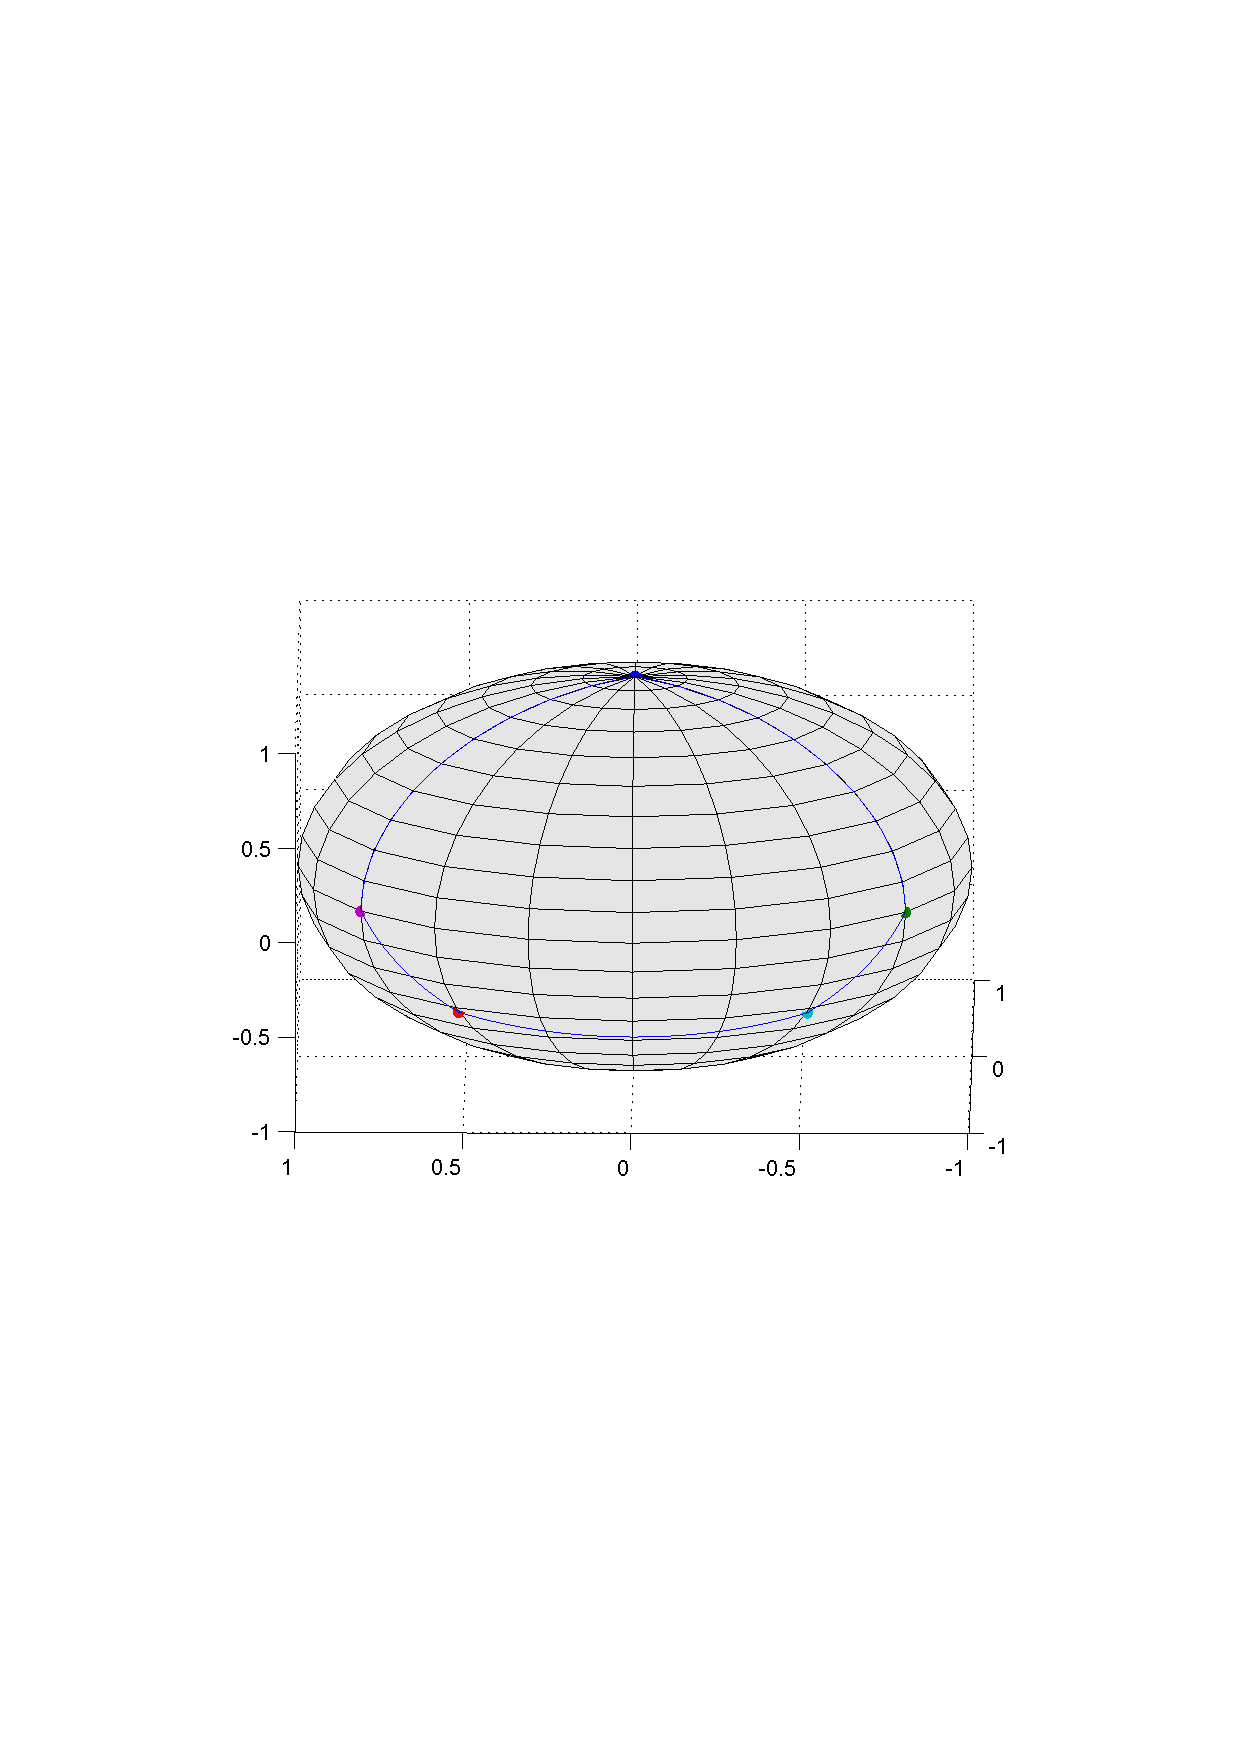
\includegraphics[scale=0.6]{penta1.png}
\caption{Pentagram 1 plotted on the Bloch sphere}
\label{fig:penta1}
\end{center}
\end{figure}
\\
Remember that a phase $\pi$ does not change the vectors. Now that the pentagram is understood, the inequality can be tackled. 

Since the only interesting solutions are those that exist on the spheres surface, that is to say that the vectors are normalized, $a_0^2+a_1^2+a_2^2=1$. These solutions can be simply visualized below. The question now arises if the violation inside or outside of the area?

Using any mathematical software to calculate the minimum value of the function of the left of the inequality, the minimum value is found as $-3.73559$ when $(a_0,a_1,a_2)$=(0,0.821597,-0.570069). This means that the inequality is violated atleast at this point which is \textbf{inside} the area. However it can be seen that the point is not inside our pentagram, this can be seen, either in the subsection above or below where the pentagram and area are plotted at the same time.
Now it must be seen if there exists an area inside the pentagon where the inequality is violated. 

\begin{figure}[h!]
\begin{center}
\includegraphics[scale=0.5]{ine1.png}
\caption{The first pentagram inequality plotted on the Bloch sphere}
\label{fig:ine1}
\end{center}
\end{figure}
\newpage
\subsection{Violation of the inequality}\label{subsec:Violation of the inequalit}
By plotting the pentagram and the inequality in the same graph it can be seen where this area exists. See the simple plot below.
The dots are an outline of the area, in which the inequality is violated. As can be seen, there is an overlap between the pentagram and the inequality. There is also another area outside of the pentagram, this is excluded due to it being uninteresting since the quantum mechanical part excludes this area.
The observant will notice that since a phase shift of $\pi$ is unimportant there will of course be an identical area on the opposite side of the sphere. Everything that follows can be translated to that area by using a phase shift of $\pi$. There is a big overlap of the inequality and the pentagram, the parts that are not covered, can they be covered by other inequalities from other pentagrams? Otherwise there exists states that violate the pentagram inequality.
\begin{figure}[H]
\begin{center}
\includegraphics[scale=0.5]{sphere1ine.png}
\caption{Pentagram 1 with its inequality}
\end{center}
\end{figure}
\newpage
\section{Producing more pentagrams}\label{sec:Producing more pentagrams}
Starting with the simplest second pentagon. Given the vectors in~\subsectionref{subsec:Choosing vectors}, there is another pentagram that can be created, using the following vectors:
\begin{equation*}
|\psi2_1>=
\begin{pmatrix}
0.3892\\
-0.2847\\
0.8761\\
\end{pmatrix}
,
|\psi2_2>=
\begin{pmatrix}
0.0000\\
0.9511\\
0.3090\\
\end{pmatrix}
,
|\psi2_3>=
\begin{pmatrix}
-0.3892\\
-0.2847\\
0.8761\\
\end{pmatrix}
,
|\psi2_4>=
\begin{pmatrix}
0.7071\\
0.5172\\
0.4822\\
\end{pmatrix}
,
\end{equation*}
\begin{equation*}
|\psi2_5>=
\begin{pmatrix}
-0.7071\\
0.5172\\
0.4822\\
\end{pmatrix}
\end{equation*}
Using these vectors, the exact same procedure as in~\subsectionref{subsec:Pentagram produced by the vectors} is used. First a pentagon is produced, then the inequality is calculated with these vectors. See the pictures below 
\begin{figure}[H]
\begin{center}
\includegraphics[scale=0.6]{penta2.png}
\caption{Pentagram 2 plotted on the Bloch sphere}
\label{fig:penta2}
\end{center}
\end{figure}
Now the inequality is plotted in the same picture.
\begin{figure}[H]
\begin{center}
\includegraphics[scale=0.6]{sphere2ine.png}
\caption{Pentagram 2 with its inequality}
\end{center}
\end{figure}
By plotting the two inequalities together it is shown that their areas do overlap, as seen below.
\begin{figure}[H]
\begin{center}
\includegraphics[scale=0.5]{ine12.png}
\caption{Pentagon 1 and 2 with their inequalities}
\end{center}
\end{figure}
To see if there is any part of the first pentagram not covered, the two inequalities are plotted over the first pentagram.
\begin{figure}[H]
\begin{center}
\includegraphics[scale=0.5]{penta1ine12.png}
\caption{Pentagon 1 with the inequality from 1 and 2}
\end{center}
\end{figure}
It can be seen in the later figure that four arms of the pentagram is uncovered by the pentagram, what must be remembered is that the interest lies at what part of the sphere is covered by the inequalities. This means that the only interest of the pentagram is to create the inequalities.


Now it must be seen what other pentagons can be created and what the inequality looks like in all of these.
One might think that this seem like a lot of unnecessary work, since it is the same inequality which should simply rotate with the pentagram. \textbf{This may however not be the case}, due to the fact that the inequality depends on the vectors used to produce the pentagram. This means that the inequality may not fill the sphere as expected. Also, the first rotation will be along an axis but not the second.
\newpage
\section{Producing even more pentagrams}
As discussed, take more vectors from~\cite{Kochen1968The} which can be represented as a rotation of our first vectors $18^\circ$ around the x-axis or around the vector: 
\begin{equation*}
\begin{pmatrix}
1\\
1\\
1\\
\end{pmatrix}
\end{equation*}
will produce more inequalities.
To start, rotate the inequalities that were discussed around the x-axis. If this produces a band that covers the entire sphere, and the point (1,1,1) then everything is done.
For simplicity, start with the rotation $18^\circ$ around the x-axis. For an easier plot, only the inequalities from the two first pentagrams are presented.
\begin{figure}[H]
\begin{center}
\includegraphics[scale=0.5]{ine12all.png}
\caption{The inequalities rotated around the x-axis.}
\label{fig:ine12all}
\end{center}
\end{figure}
It is seen that the the second inequalities are covered by the first, also the first inequalities create a band. Now the question is: Is the vector (1,1,1) inside the band? This is of importance since if it is then rotating the band around this point will cover the entire sphere. If not, then it must be seen if any rotated inequality can cover this point. First visually then using the formula from the appendix to calculate the inequality in the first pentagram. Remember the vectors given in~\ref{sec:Pentagram produced by the vectors} which in the inequality produced~\eqref{eq:Area}. Inputting the vector (1,1,1) normalized with the factor $\frac{1}{\sqrt{3}}$ will result in $-3.0349 \geq -3$ which is false! Thus is it inside the inequality, see below.
\begin{figure}[H]
\begin{center}
\includegraphics[scale=0.5]{ine12all111.png}
\caption{The inequalities rotated around the x-axis with the 111 vector plotted.}
\label{fig:ine12all111}
\end{center}
\end{figure}

Calculate where the inequalities meet and see where the thinnest band is produced. By taking the scalar product between the overlap vectors an angle can be calculated, it is  this that will be used to create the band. Below a picture is presented of how three inequalities overlap and also where the vectors must be. 
\begin{figure}[H]
\begin{center}
\includegraphics[scale=0.5]{overlap114.png}
\caption{Three inequalities plotted.}
\label{fig:overlap114}
\end{center}
\end{figure}
It is seen that the band is equally narrow both above and below. 
\begin{figure}[H]
\begin{center}
\includegraphics[scale=0.5]{band.png}
\caption{A plot of there limits to the band.}
\label{fig:band}
\end{center}
\end{figure}
Using the points above, one can draw small circles around the sphere. This is done by taking the x-coordinates from the intersection and plotting the following 
\begin{equation}
0.5812^2+y^2+z^2=1
\end{equation}
This is shown in the plot below with the point (1,1,1) visible.
\begin{figure}[H]
\begin{center}
\includegraphics[scale=0.5]{completeband111big.png}
\caption{A plot of the band with the point (1,1,1)}
\label{fig:completeband}
\end{center}
\end{figure}
It can be seen above that the point (1,1,1) is inside the band. This is also seen from normalizing it and using the equation above (since $\frac{1}{\sqrt{3}}=0.5774<0.5812<1$
Since rotations are done around this point this means that the bands created by rotating the inequalities around will cover all points on the sphere if there is enough of an overlap between the rotated bands. 
\subsection{In the sphere covered?}\label{Is the sphere covered?}
As discussed in the previous subsection, if there is enough of an overlap between the rotated bands, then it is known that the sphere is covered and thus the goal of this thesis has been reached.
All three rotated bands can be seen in the figure below, here it is seen how the whole sphere is covered.
\begin{figure}[H]
\begin{center}
\includegraphics[scale=0.9]{coveredsphere.png}
\caption{The sphere covered with bands created by the inequalities}
\label{fig:coveredsphere}
\end{center}
\end{figure}

\chapter{Discussion}\label{cha:discussion}
\newpage
\section{Was the sphere covered by inequalities?}
As seen in figure~\ref{fig:coveredsphere} and discussed in~\subsectionref{Is the sphere covered?} it seems that the whole sphere is covered by these inequalities. Through the whole thesis there have been signs and proof that this may be the case, however it was only fully seen at the end. What does this imply? 
\subsection{What does this imply?}
If the whole Bloch sphere is either inside or on the border of the inequalities as seen in the thesis, this means that all possible states of a spin 1 system can be explained by the details given in the article~\cite{PhysRevLett.101.020403}. This means that the inequality posed is always violated  and that quantum mechanics can be used to explain the spin 1 system.
Two questions arise from this.\\
It says all states above, but is this really true?\\
Has it then been shown that all possible states of a spin 1 system can be explained by the details given in the article~\cite{PhysRevLett.101.020403}?\\
The answer to both of these questions is no.\\
There were a few restrictions given in the start of this thesis. Remember that to be able to visualize the states simply the Bloch sphere was used. However it can not be used for a spin 1 system, unless only real coefficients for the vectors that represent the states are used. This was a restriction that has been used throughout the thesis. It is quite undeniable that a proof that the inequality covers all of the real states has been found in this thesis, however nothing has been said about those which require a complex representation. Therefore, it can be said that the non-contextual inequality given in the article~\cite{PhysRevLett.101.020403} is violated for all of the real states that exist for a spin 1 system. To say anything else would require more research.


\chapter{Conclusions}\label{cha:conclusions}
\newpage
\section{Conclusion}
As seen in figure~\ref{fig:coveredsphere} and discussed in~\subsectionref{Is the sphere covered?} and in \chapterref{cha:discussion} it seems that the whole sphere is covered by these inequalities when the restriction of real coefficients is applied to the states.  

\section{Further research to be done}
\subsection{Calculating with complex coefficients}
By removing the requirement that all states only should have real coefficients would open up a whole new world. One would unfortunately lose the simple visualization, as was preferred in this thesis, however it would give the full set of states that exist. This would not require much more than was done in this thesis, simply recalculate the inequalities with complex coefficients and then in some way try to visualize if this covers the full set of states. 
\subsection{Other spin systems}
As discussed previously, mostly spin $\frac{1}{2}$ systems are of interest and in this thesis spin 1 systems were discussed. However there exists a whole range of spin systems, almost all half integers and all integers have their own spin system in nature. Is there any schema that can include these? This is an interesting question that could be seen as further research from this thesis.

\part*{Appendix}
\appendix
\chapter{Calculations}\label{cha:Calculations}
\section{Finding the non-contextual area}
A notation used in this appendix, $\identity_x$ is known as the Identity matrix, with dimension x. \\
By taking the operators $A_i$ as projector operators, then the operator can be written as 
\begin{equation} \label{eq:Defop}
A_i = \identity_3 - 2 |\psi_i><\psi_i|  
\end{equation}
To be able to calculate where the inequality may be unfulfilled, a state in a given place on the sphere must be taken.
For instance, taking a state 
\begin{equation}
|\psi> = a_0|-1>+a_1|0>+a_2|1> 
\end{equation}
Remember from the introduction~\subsectionref{subsec:Dirac bra-ket notation}
\begin{equation}
|\psi>^\dagger = <\psi|=a_0^\dagger<-1|+a_1^\dagger<0|+a_2^\dagger<1| 
\end{equation}
Also it is important to remember that each of the taken states have been normalized and fulfil the following property:
\begin{equation}
<\psi|\psi> = a_0^2+a_1^2+a_2^2 = 1 
\end{equation}
The states used can be seen Cartesian unit vectors. To start with a simple case, which will be the case looked at in this thesis, let $a_i$ be real numbers, and using that $|\psi_i>$ was given in ~\subsectionref{subsec:Pentagon produced by the vectors}.

Using these, equation~\ref{eq:Inequality} 
\begin{equation*}
\langle A_1 A_2 \rangle + \langle A_2 A_3 \rangle + \langle A_3 A_4 \rangle + \langle A_4 A_5 \rangle +
\langle A_5 A_1 \rangle \geq -3
\end{equation*}
can be calculated by using the property
\begin{equation} 
\langle A_1 A_2 \rangle = <\psi|A_1 A_2|\psi>
\end{equation} 
This can be done through some ordinary linear algebra since we take the states as our basis vectors for our space. Also, not to forget that we defined the properties of the operators above, see equation~\ref{eq:Defop}. Since the vectors chosen in the operators, $|\psi_i>$, are pairwise orthogonal; the calculations seen below are almost trivial:
\begin{equation}
\begin{aligned}
<\psi|A_1 A_2|\psi>=(a_0<-1|+a_1<0|+a_2<1|)(\identity_3-2|\psi_1><\psi_1|)(\identity_3-2|\psi_2><\psi_2|)*
\\(a_0|-1>+a_1|0>+a_2|1>)
\\=(a_0<-1|+a_1<0|+a_2<1|)*(\identity_3-2|\psi_1><\psi_1|-2|\psi_2><\psi_2|)*
\\(a_0|-1>+a_1|0>+a_2|1>)
\\=(a_0<-1|+a_1<0|+a_2<1|)*((a_0|-1>+a_1|0>+a_2|1>)
\\-2a_2|1>-2(-0.5904a_0-0.8071a_1)|\psi_2>)
\\=1-2a_2^2-2(-0.5904a_0-0.8071a_1)^2
\end{aligned}
\end{equation}
Where in the last step the normality condition was used. Now the other calculations will be similar, the results and a few steps in the calculations are presented below.
\begin{multline}
<\psi|A_2 A_3|\psi>=(a_0<-1|+a_1<0|+a_2<1|)*(\identity_3-2|\psi_2><\psi_2|-2|\psi_3><\psi_3|)*
\\(a_0|-1>+a_1|0>+a_2|1>)=1-2(-0.5904a_0-0.8071a_1)^2-
\\2(0.7071a_0-0.5172a_1-0.4822a_2)^2
\\
<\psi|A_3 A_4|\psi>=(a_0<-1|+a_1<0|+a_2<1|)*(\identity_3-2|\psi_3><\psi_3|-2|\psi_4><\psi_4|)*
\\(a_0|-1>+a_1|0>+a_2|1>)=1-2(0.7071a_0-0.5172a_1-0.4822a_2)^2-
\\2(-0.7071a_0-0.5172a_1-0.4822a_2)^2
\\
<\psi|A_4 A_5|\psi=(a_0<-1|+a_1<0|+a_2<1|)*(\identity_3-2|\psi_4><\psi_4|-2|\psi_5><\psi_5|)*
\\(a_0|-1>+a_1|0>+a_2|1>)=1-2(-0.7071a_0-0.5172a_1-0.4822a_2)^2-
\\2(0.5904a_0-0.8071a_1)^2
\\
<\psi|A_5 A_1|\psi>=(a_0<-1|+a_1<0|+a_2<1|)*(\identity_3-2|\psi_5><\psi_5|-2|\psi_1><\psi_1|)*
\\(a_0|-1>+a_1|0>+a_2|1>)=1-2(0.5904a_0-0.8071a_1)^2-2a_2^2
\end{multline}
Or a more general formula, with index i,j where the corresponding vectors are orthogonal, would be
\begin{equation}
\begin{aligned}
<\psi|A_i A_j|\psi>=
1-2<\psi|\psi_i><\psi_i|\psi>-2<\psi|\psi_j><\psi_j|\psi>
\end{aligned}
\end{equation}
After all this the inequality can be written as 
\begin{dmath}
1-2a_2^2-2(-0.5904a_0-0.8071a_1)^2+1-2(-0.5905a_0-0.8071a_1)^2-
2(0.7071a_0-0.5172a_1-0.4822a_2)^2+
1-2(0.7071a_0-0.5172a_1-0.4822a_2)^2-
2(-0.7071a_0-0.5172a_1-0.4822a_2)^2 +
1-2(-0.7071a_0-0.5172a_1-0.4822a_2)^2-
2(-0.5904a_0+0.8071a_1)^2+1-2(-0.5904a_0+0.8071a_1)^2-2a_2^2
\geq -3
\end{dmath}
This is rewritten as the following:
\begin{dmath}\label{eq:Area1}
5-4a_2^2-4(-0.5904a_0-0.8071a_1)^2-4(0.7071a_0-0.5172a_1-0.4822a_2)^2
-4(-0.7071a_0-0.5172a_1-0.4822a_2)^2-4(-0.5904a_0+0.8071a_1)^2 \geq -3
\end{dmath}
It is quite easy to see the generalization of this, as has been used in the thesis, though it is left to the reader to fill in the blanks them selves.
This is all which is discussed in this appendix section.

%\include{rtthesis-doc}
%\backmatter
\nocite{Grund}
\bibliography{myrefs}
\printindex
\end{document}
